\documentclass[12pt]{article}
\usepackage{amsmath}
\usepackage{amssymb}
\usepackage{graphicx}
\usepackage{subcaption}
\usepackage{hyperref}
\usepackage{multicol}
\usepackage[latin1]{inputenc}
\usepackage{listings}
\usepackage{scrextend}

\usepackage{changepage} %Adjustwidth
\usepackage[margin=1in]{geometry}

\usepackage{algorithm}
%\usepackage{algorithmic}
\usepackage{algpseudocode}
\usepackage{alltt}


% Used for code blocks ----------------------------------------------------------------
\usepackage{color}
\usepackage{xcolor}
\usepackage{listings}

\usepackage{caption}
\DeclareCaptionFont{white}{\color{white}}
\DeclareCaptionFormat{listing}{\colorbox{gray}{\parbox{\textwidth}{#1#2#3}}}
\captionsetup[lstlisting]{format=listing,labelfont=white,textfont=white}
% -----------------------------------------------------------------------------------------



\title{ComS 342\\Recitation 2, 10:00 Tuesday\\Homework 9}
\author{Sean Gordon}
%\date{09/09/2019}

\begin{document}
\maketitle


\hrulefill \\


\begin{center}
\noindent 1) Z = [1, 4, 6, 3, 6].
\end{center}


\hrulefill \\


\begin{multicols}{2}

\noindent 2a)\\\\
fib(0, 0).\\
fib(1, 1).\\\\
fib(N, Res) :-\\
\indent N $>$ 1,\\
\indent N1 is N-1,\\
\indent N2 is N-2,\\\\
\indent fib(N1, R1),\\
\indent fib(N2, R2),\\\\
\indent Res is R1+R2.\\

\columnbreak

\noindent 2b)\\\\
rev(L, Res) :-\\
\indent revHelper(L, [ ], Res).\\\\
revHelper([ ], Accum, Accum).\\
revHelper([H$|$T], Accum, Res) :-\\
\indent number(H),\\
\indent revHelper(T, [H$|$Accum], Res);\\\\
\indent revHelper(H, [ ], Temp),\\
\indent revHelper(T, [Temp$|$Accum], Res).\\

\end{multicols} 


\hrulefill \\
\pagebreak


\noindent 3a)\\
sentence([ ]).\\
sentence(S) :- s(S, [ ]).\\

\noindent s(L1, L2) :- f(L1, L2).\\
s(L1, L4) :- t(L1, L2), n(L2, L3), t(L3, L4).\\

\noindent f(L1, L5) :- if(L1, L2), b(L2, L3), then(L3, L4), s(L4, L5).\\
\noindent f(L1, L7) :- if(L1, L2), b(L2, L3), then(L3, L4), s(L4, L5), else(L5, L6), s(L6, L7).\\

\noindent b(L1, L4) :- t(L1, L2), e(L2, L3), t(L3, L4).\\

\noindent if([if$|$Tail], Tail).\\
then([then$|$Tail], Tail).\\
else([else$|$Tail], Tail).\\

\noindent t([x$|$Tail], Tail).\\
t([y$|$Tail], Tail).\\
t([z$|$Tail], Tail).\\
t([1$|$Tail], Tail).\\
t([0$|$Tail], Tail).\\

\noindent e([$<$$|$Tail], Tail).\\
e([$>$$|$Tail], Tail).\\

\noindent n([+$|$Tail], Tail).\\
n([-$|$Tail], Tail).\\
n([=$|$Tail], Tail).\\\\


\noindent 3b) sentence(X)? Exceeds memory due to S $<$-$>$ F recursion. I'm confused.
\begin{figure}[h!]
	\centering
	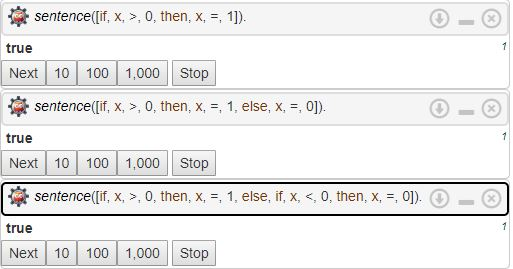
\includegraphics[width=100mm,scale=1]{Q3b.JPG}
\end{figure}

\noindent 3c) Yes, sub-goal order matters as they are executed sequentially.\\



\pagebreak
\hrulefill \\

\noindent 4) \\
\% House: [Color, Man, Pet, Drink, Cig]\\
next(A, B, L):-nextto(A, B, L) ; nextto(B, A, L).\\
write\_list(L):-forall(member(Mem, L), (write(Mem), nl)).\\

\noindent start(Houses):- length(Houses, 5), \\
    member([red, english, \_, \_, \_], Houses), \\
	member([\_, spaniard, dog, \_, \_], Houses), \\
    member([green, \_, \_, coffee, \_], Houses), \\
    member([\_, ukranian, \_, tea, \_], Houses), \\
    
\noindent next([ivory, \_, \_, \_, \_], [green, \_, \_, \_, \_],  Houses), \\
    
\noindent member([\_, \_, snails, \_, oldGold], Houses), \\
    member([yellow, \_, \_, \_, kools], Houses), \\
    
\noindent Houses= [\_, \_, [\_, \_, \_, milk, \_], \_, \_], \\
    Houses= [[\_, norwegian, \_, \_, \_], \_, \_, \_, \_], \\
    
\noindent next([\_, \_, \_, \_, camel], [\_, \_, fox, \_, \_],  Houses), \\
    next([\_, \_, \_, \_, kools], [\_, \_, horse, \_, \_],  Houses), \\
    
\noindent member([\_, \_, \_, orangeJuice, luckyStrike], Houses), \\
    member([\_, japanese, \_, \_, parliaments], Houses), \\
    
\noindent next([\_, norwegian, \_, \_, \_], [blue, \_, \_, \_, \_],  Houses), \\
    
\noindent member([\_, \_, \_, water, \_], Houses), \\
    member([\_, \_, zebra, \_, \_], Houses), \\
    
\noindent write\_list(Houses).\\\\


\noindent After running ``start(S),fail.'', the below list is printed:\\\\
$[$yellow, norwegian, fox,     water,  	       kools$]$\\
$[$blue,    ukranian,     horse, tea,               camel$]$\\
$[$red,     english,        snails,  milk,  	       oldGold$]$\\
$[$ivory,  spaniard,      dog,    orangeJuice, luckyStrike$]$\\
$[$green, japanese,    zebra,  coffee,          parliaments$]$\\

\noindent Therefore, the norwegian drinks water, and the japanese owns the zebra.

\end{document}
















